\documentclass{article}

\usepackage{amsmath}
\usepackage{enumitem}
\usepackage{tikz-timing}
\usepackage{graphicx}

\graphicspath{{./images/}}

\begin{document}
	
	
	2.2. Explain what are the differences between latches and flip flops with your own words. \\
	The main difference between a latch and a flip flop is that the first is asynchronous, and the second is synchronized with a clock. When, for instance, a set signal is given to latch, the time required to switch states will only depend on the internal delays of gate. Flip flops, however, are triggered either by positive or negative edge of clock signal, according to their type. Implementation of synchronization requires more logic gates. \\
		
 	2.4. Construct the truth table of an SR latch which does not have an Enable input. 
 	
 	\begin{center} 
 	\begin{tabular}{|c|c|c|c|}
	 	\hline
	 	\rule{0pt}{1\normalbaselineskip}S & R & $Q(t+1)$ & $\overline{Q}(t+1)$ \\
		\hline	
		\rule{0pt}{1\normalbaselineskip}0 & 0 & $Q(t)$ & $\overline{Q}(t)$ \\
		1 & 0 & 1 & 0 \\
		0 & 1 & 0 & 1 \\
		1 & 1 & $x$ & $x$ \\
		\hline
	\end{tabular}
	\begin{tabular}{r}
	\rule{0pt}{1\normalbaselineskip}\\
	\rule{0pt}{1\normalbaselineskip}(preserve)\\
	(set)\\
	(reset)\\
		(forbidden) \\
	\end{tabular}
	\end{center}
	where $Q(t)$ and $Q(t+1)$, $\overline{Q}(t)$ and $\overline{Q}(t+1)$ represent previous and next states, and $x$ is unknown. \\
	
	2.6. Construct the truth table of a D flip flop.	\\
	\begin{center} 
 	\begin{tabular}{|c|c|c|c|}
	 	\hline
		\rule{0pt}{1\normalbaselineskip}D & CLK & $Q(t+1)$ &  $\overline{Q}(t+1)$ \\
		\hline	
		\rule{0pt}{1\normalbaselineskip}$\phi$ & $\phi$ & $Q(t)$ & $\overline{Q}(t)$ \\
		1 & \texttiming{LH} & 1 & 0 \\
		0 & \texttiming{LH} & 0 & 1 \\
		\hline
	\end{tabular}
	\begin{tabular}{r}
	\rule{0pt}{1\normalbaselineskip}\\
	\rule{0pt}{1\normalbaselineskip}(preserve)\\
	(set)\\
	(reset)\\
	\end{tabular}
	\end{center}
	
	where $Q(t)$ and $Q(t+1)$, $\overline{Q}(t)$ and $\overline{Q}(t+1)$ represent previous and next states, $\phi$ is any state and \texttiming{LH} symbol means rising edge, i.e. transition from low to high. \\
	
	\newpage

	\textbf{Part 1:}
	\begin{figure}[h]
		\centering
		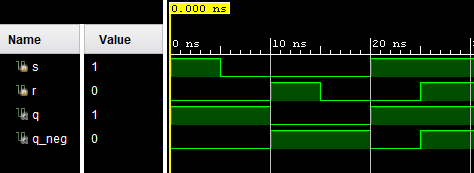
\includegraphics[width=0.8\textwidth]{part1.png}
		\caption{SR Latch simulation}
		\centering
	\end{figure}	
	
	The behaviour of SR Latch can be expressed with an equation of form $Q(t + 1) = f(S; R; Q(t)).$ From the truth table, all combinations of S and R are selected except the forbidden state, and $Q(t + 1)$ is expressed and simplified using rules of Boolean algebra as follows:

	\begin{align*}			 
	 Q(t + 1) &= \bar{S} \bar{R} Q(t) + \bar{S} R \cdot 0 + S \bar {R} \cdot 1 \tag{Truth table} \\
	 &= \bar{S} \bar{R} Q(t) + 0 + S  \bar{R} \cdot 1 \tag{Dominance} \\
	 &= \bar{S} \bar{R} Q(t) + S  \bar{R} \tag{Identity} \\
	 &= \bar{S} \bar{R} Q(t) + S \bar{R} + \bar{R} \bar{R} Q(t) \tag{Consensus theorem} \\
	 &= \bar{S} \bar{R} Q(t) + S \bar{R} + \bar{R} Q(t) \tag{Idempotency} \\
	 &=  Q(t)(\bar{S} \bar{R} + \bar{R}) + S \bar{R}  \tag{Distributivity} \\
	 &=  Q(t)\bar{R} + S \bar{R}  \tag{Absorption} \\
	 &=  Q(t)\bar{R} + S\\
	\end{align*}

	In the final step, $\bar{R}$ is omitted because state $S = 1, R = 1$ is forbidden and should never happen. Therefore omitting it does not change the truth table. To summarize, SR Latch's output is $1$ whenever S is on and R is off, is $0$ whenever R is on and S is off, and it maintains the previous state if both S and R go low. It is therefore called a memory circuit. \\

	\newpage
	
	\textbf{Part 3:}
	\begin{figure}[h]
		\centering
		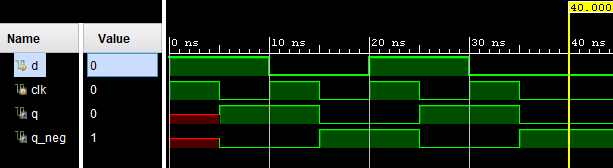
\includegraphics[width=0.8\textwidth]{part3.png}
		\caption{Negative edge triggered D flip-flop simulation}
		\centering
	\end{figure}	
	
	As it is seen from the wave form, D flip-flop can change state only on the falling clock edge.

\newpage

	\textbf{Part 6:}
	\begin{figure}[h]
		\centering
		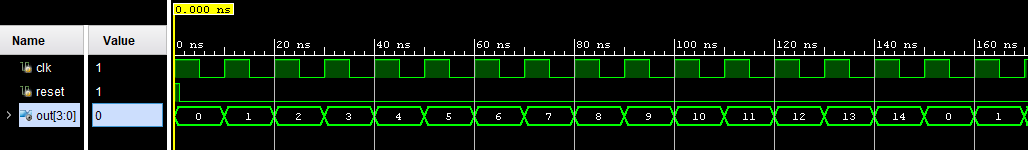
\includegraphics[width=1\textwidth]{part6.png}
		\caption{Synchronous up counter simulation}
		\centering
	\end{figure}	
	
	The truth table is as follows:\\

	\begin{tabular}{|c|c|c|c|}
	\hline
	\rule{0pt}{1\normalbaselineskip} CLK & Reset & $\{A_3, A_2, A_1, A_0\}$ &  $\{A_3, A_2, A_1, A_0\}^+$ \\\hline
	$\phi$ & \texttiming{LH} & $\{\phi,\ \ \phi,\ \  \phi,\ \  \phi\}$ & $\{0,\ \ 0,\ \ 0,\ \  0\}$\\ 
	\texttiming{LH} & 0 & $\{0,\ \ 0,\ \ 0,\ \  0\}$ & $\{0,\ \ 0,\ \ 0,\ \  1\}$\\ 
	\texttiming{LH} & 0 & $\{0,\ \ 0,\ \ 0,\ \  1\}$ & $\{0,\ \ 0,\ \ 1,\ \  0\}$\\ 
	\texttiming{LH} & 0 & $\{0,\ \ 0,\ \ 1,\ \  0\}$ & $\{0,\ \ 0,\ \ 1,\ \  1\}$\\ 
	\texttiming{LH} & 0 & $\{0,\ \ 0,\ \ 1,\ \  1\}$ & $\{0,\ \ 1,\ \ 0,\ \  0\}$\\ 
	\texttiming{LH} & 0 & $\{0,\ \ 1,\ \ 0,\ \  0\}$ & $\{0,\ \ 1,\ \ 0,\ \  1\}$\\ 
	\texttiming{LH} & 0 & $\{0,\ \ 1,\ \ 0,\ \  1\}$ & $\{0,\ \ 1,\ \ 1,\ \  0\}$\\ 
	\texttiming{LH} & 0 & $\{0,\ \ 1,\ \ 1,\ \  0\}$ & $\{0,\ \ 1,\ \ 1,\ \  1\}$\\ 
	\texttiming{LH} & 0 & $\{0,\ \ 1,\ \ 1,\ \  1\}$ & $\{1,\ \ 0,\ \ 0,\ \  0\}$\\ 
	\texttiming{LH} & 0 & $\{1,\ \ 0,\ \ 0,\ \  0\}$ & $\{1,\ \ 0,\ \ 0,\ \  1\}$\\ 
	\texttiming{LH} & 0 & $\{1,\ \ 0,\ \ 0,\ \  1\}$ & $\{1,\ \ 0,\ \ 1,\ \  0\}$\\ 
	\texttiming{LH} & 0 & $\{1,\ \ 0,\ \ 1,\ \  0\}$ & $\{1,\ \ 0,\ \ 1,\ \  1\}$ \\ 
	\texttiming{LH} & 0 & $\{1,\ \ 0,\ \ 1,\ \  1\}$ & $\{1,\ \ 1,\ \ 0,\ \  0\}$  \\ 
	\texttiming{LH} & 0 & $\{1,\ \ 1,\ \ 0,\ \  0\}$ & $\{1,\ \ 1,\ \ 0,\ \  1\}$  \\ 
	\texttiming{LH} & 0 & $\{1,\ \ 1,\ \ 0,\ \  1\}$ & $\{1,\ \ 1,\ \ 1,\ \  0\}$  \\ 
	\texttiming{LH} & 0 & $\{1,\ \ 1,\ \ 1,\ \  0\}$ & $\{0,\ \ 0,\ \ 0,\ \  0\}$  \\ 
	
	\hline
\end{tabular}	
	
\newpage

\textbf{Part 7:}
	To implement pulse width modulation with a circular shift register, there must be a multiplexer which will choose between the input wave pattern and output of previous flip flop, and output the signal as input to the next flip flop. When load flag is low, flip flops behave like a circular shift register. When load flag becomes high, circular transmission is stopped and all flip flops are written to. This is the design of 2:1 multiplexer we used: \\
	\begin{figure}[h]
		\centering
		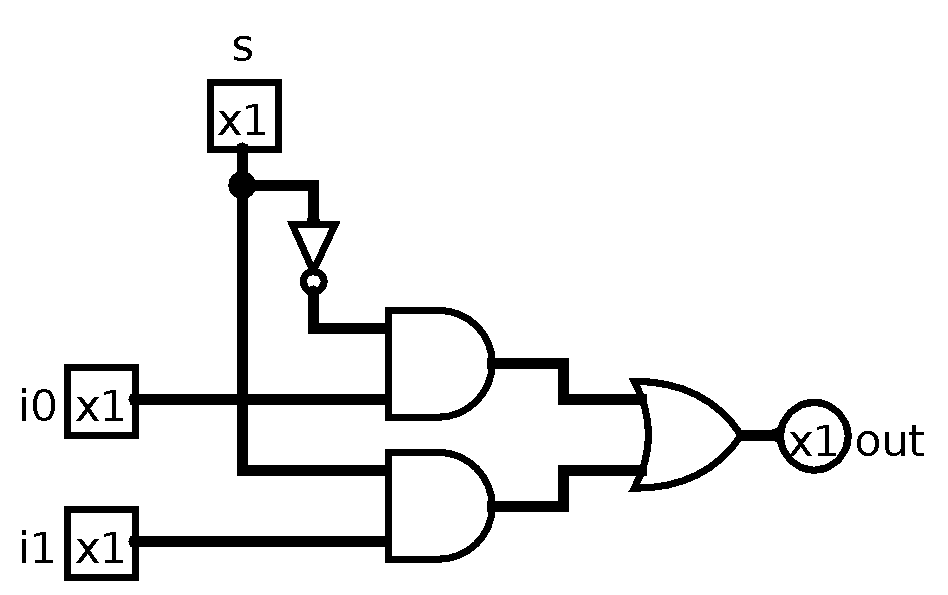
\includegraphics[width=0.6\textwidth]{mux.png}
		\caption{2:1 multiplexer design in Logisim}
		\centering
	\end{figure}	
	
It was also described and simulated with Verilog: \\	
	
	\begin{figure}[h]
		\centering
		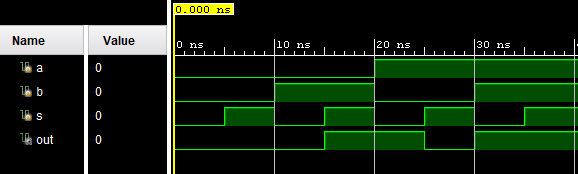
\includegraphics[width=1\textwidth]{part7_mux.png}
		\caption{2:1 multiplexer simulation in Verilog}
		\centering
	\end{figure}	
	
	The pulse generator itself is too long to fit on the page, and with that reason the following diagram is it's smaller version with same behaviour. Because D flip flops are negative edge triggered, the clock is inverted in order to make it a positive edge triggered device: \\
	
	\begin{figure}[h]
		\centering
		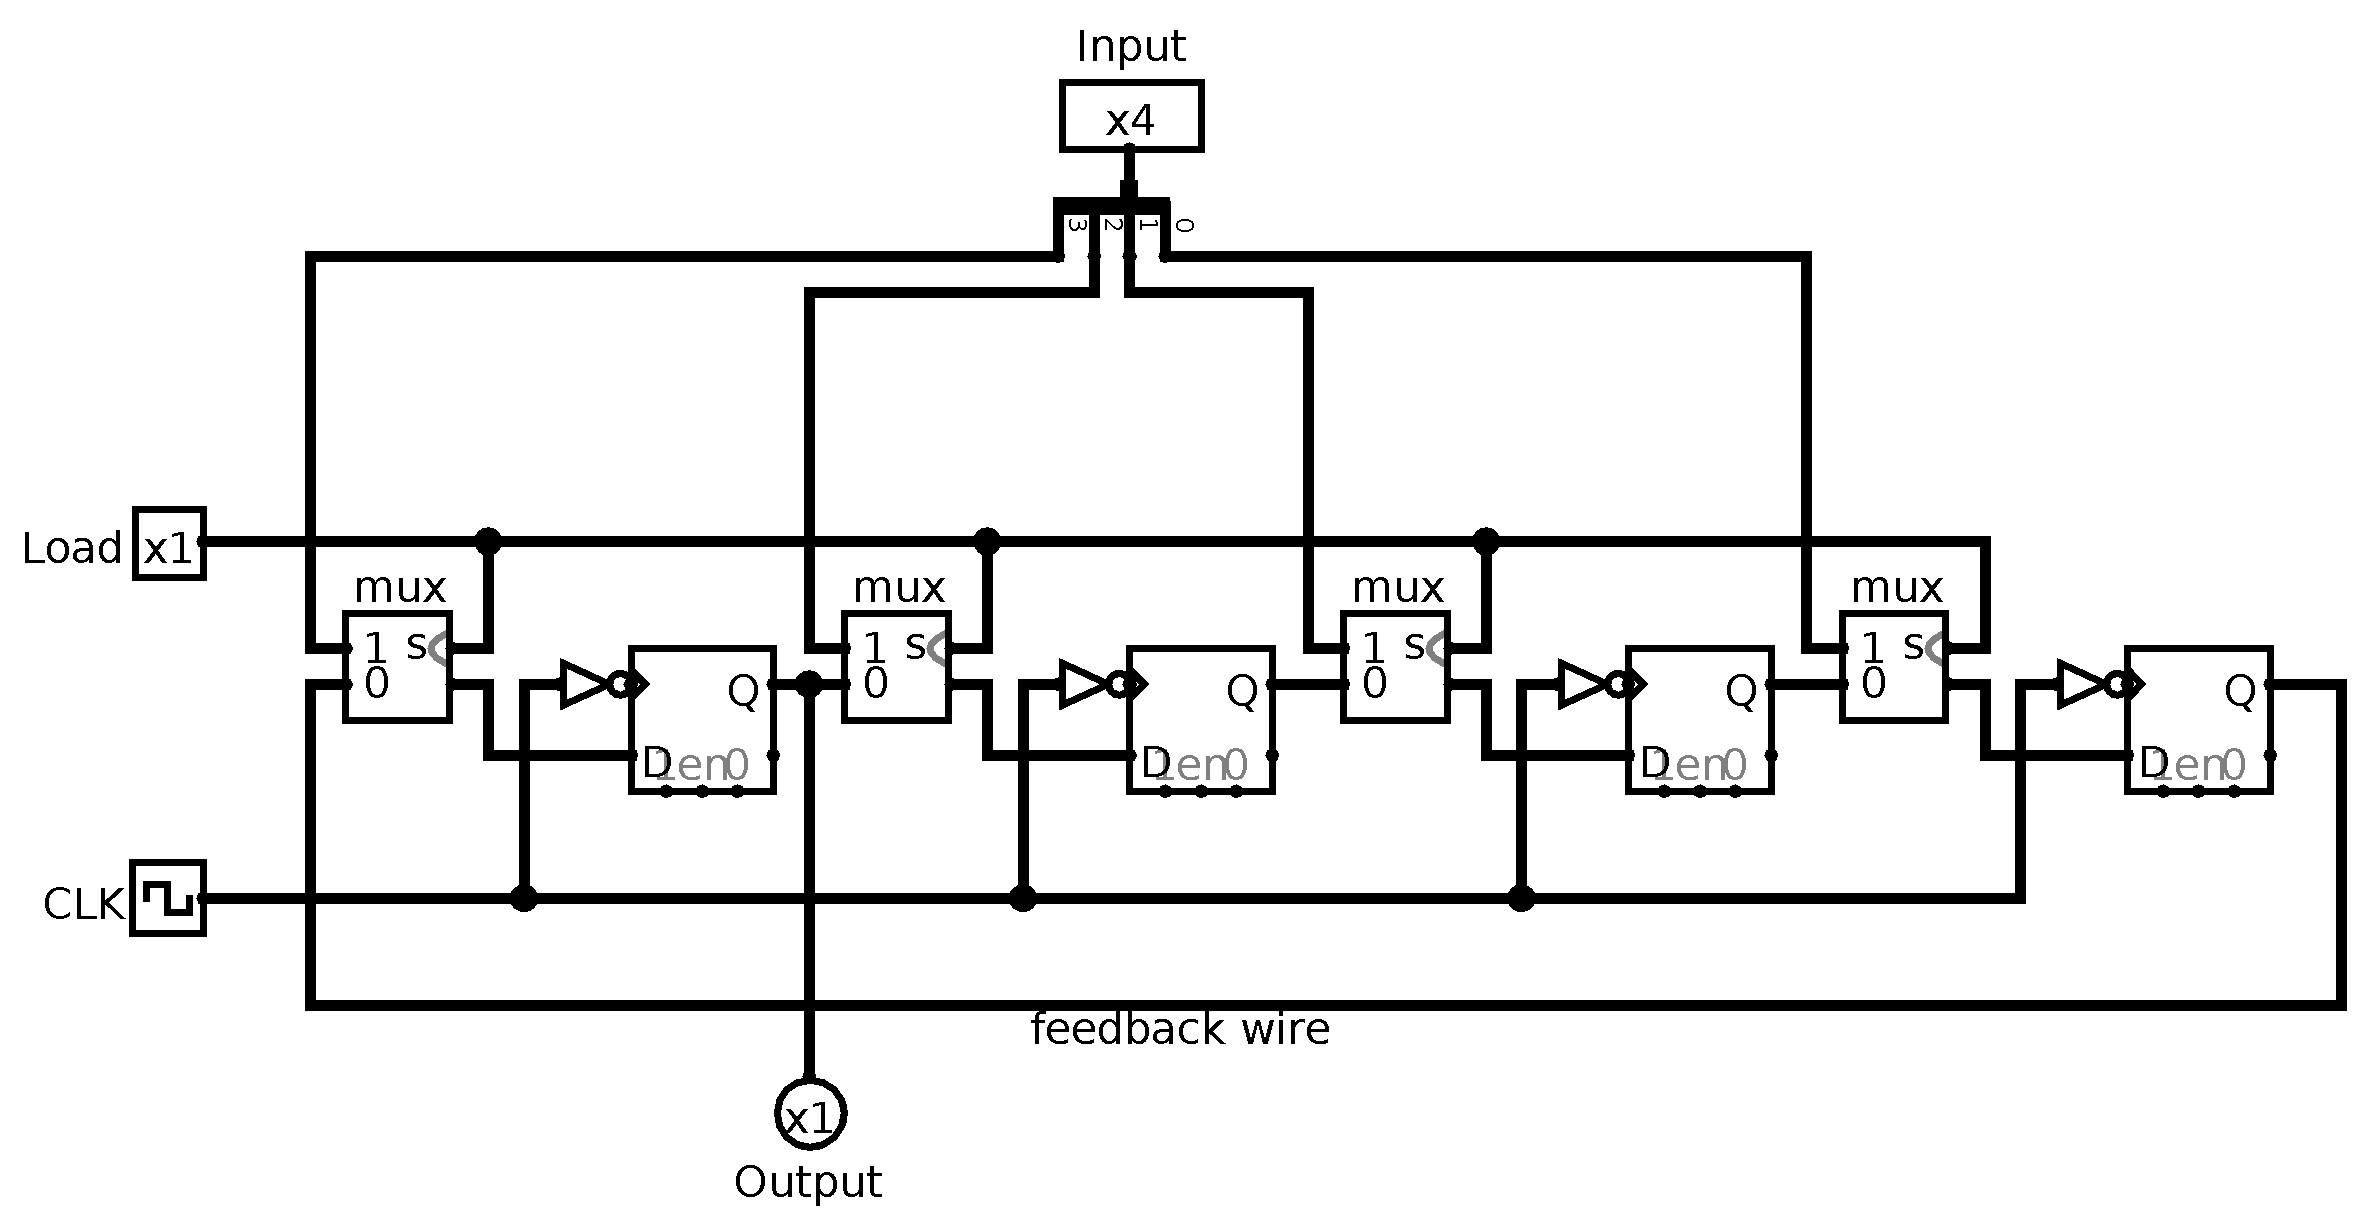
\includegraphics[width=1\textwidth]{pwm.png}
		\caption{Pulse generator design in Logisim}
		\centering
	\end{figure}	
	
	In the Verilog description we prepared, pulse generator has a 16-bit input as required. The result of simulation confirms it can deliver various pulses, such as half, quarter, one eigth of clock frequency and signals with 1/7, 3/13, 11/5 pulse-gap duration rate: \\
	
	\begin{figure}[h]
		\centering
		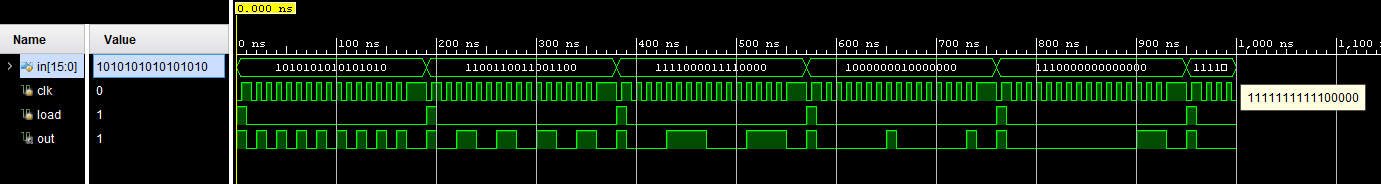
\includegraphics[width=1\textwidth]{part7.png}
		\caption{Pulse generator simulation in Verilog}
		\centering
	\end{figure}	
	

\end{document}